\documentclass{beamer}
\usepackage[utf8]{inputenc}
\usepackage{helvet}
\renewcommand{\familydefault}{\sfdefault}
\usepackage[brazil]{babel}
\usetheme{Madrid}
\usepackage{graphicx}
\usepackage{ragged2e}
\usepackage{hyperref}

\definecolor{cpsred}{RGB}{153,0,0} 
\definecolor{cpsgray}{RGB}{85,85,85} 

\usecolortheme[named=cpsred]{structure}
\setbeamercolor{title}{fg=white,bg=cpsred}
\setbeamercolor{frametitle}{fg=white,bg=cpsred}
\setbeamercolor{structure}{fg=cpsred}
\setbeamercolor{normal text}{fg=black,bg=white}
\setbeamercolor{itemize item}{fg=cpsred}

\setbeamertemplate{headline}{}

% ===================== FOOTER CUSTOM =====================
\setbeamertemplate{footline}{
    \begin{beamercolorbox}[wd=\paperwidth,ht=1.1cm,dp=3pt,leftskip=5mm,rightskip=5mm]{footline}
        \color{white}
        \raisebox{-0.1cm}{
\includegraphics[height=0.9cm]{Imagem/cpsLogo.png}}%
        \hfill \insertframenumber{} / \inserttotalframenumber
    \end{beamercolorbox}
}
\setbeamercolor{footline}{bg=cpsred, fg=white}
\setbeamertemplate{navigation symbols}{}

% ===================== CAPA =====================
\title[Criação de Camarão em Cativeiro com Monitoramento IoT para Gastronomia]{\textbf{Criação de Camarão em Cativeiro com Monitoramento IoT para Gastronomia}}
\author{}
\date{}

\begin{document}

\begin{frame}
    \centering
    \vspace{1cm}
    {\color{cpsred}\Huge\textbf{Criação de Camarão em Cativeiro com Monitoramento IoT para Gastronomia}}\\[0.8cm]
    {\Large João Kusaka / Leandro Augusto / Matheus Ferrari / Tiago Rodrigues / Victor Roder}\\[0.4cm] \textcolor{cpsgray}{Centro Paula Souza}\\[0.2cm] \textcolor{cpsgray}{FATEC Registro}
\end{frame}
% ================================================

\section{Agenda}
\begin{frame}{Agenda}
\justifying
\begin{itemize}
    \item Slide - Pitch
    \item Slide - Problematização
    \item Slide - Estado da Arte
    \item Slide - Objetivos
    \item Slide - Metodologia
    \item Slide - Apresentação prática
    \item Slide - Resultados preliminares
    \item Slide - Conclusão
\end{itemize}
\end{frame}

\section{Pitch}
\begin{frame}{Pitch}
\justifying
\end{frame}

\section{Problematização}
\begin{frame}{Problematização}
\justifying
\begin{itemize}
    \item Infraestrutura inadequada para cultivo
    \item Proliferação de doenças
    \item Falta de sistemas integrados
\end{itemize}
\end{frame}

\section{Estado da Arte}
\begin{frame}{Estado da Arte}
\justifying
\begin{itemize}
    \item Dantas, 2020 – Sistema de telemonitoramento e automação baseado em rede LoRa
    \item Udin, 2020 – Freshwater shrimp farm monitoring system for Bangladesh
    \item Zainuddin, 2019 – Water monitoring system for Vannamae shrimp cultivation
\end{itemize}
\end{frame}

\section{Objetivos}
\begin{frame}{Objetivos}
\justifying
\begin{itemize}
    \item Automatizar o controle dos cativeiros
    \item Promover eficiência e sustentabilidade
    \item Tornar o trabalho do carcinicultor mais produtivo
    \item Melhorar a qualidade do camarão
\end{itemize}
\end{frame}

\section{Metodologia}
\begin{frame}{Metodologia}
\justifying
Sensores utilizados no sistema IoT

\begin{center}
\begin{minipage}{0.32\linewidth}
    \centering
    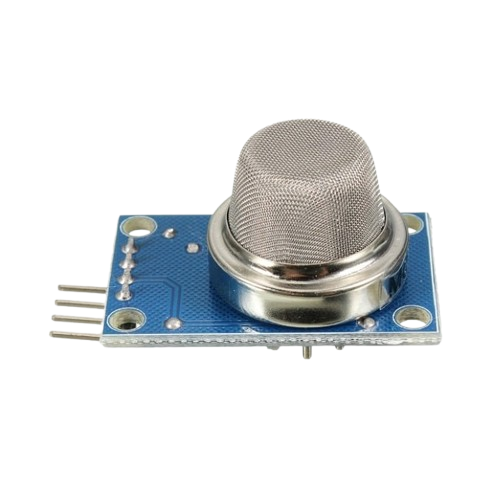
\includegraphics[width=\linewidth]{Imagem/sensorGases.png}
\end{minipage}
\begin{minipage}{0.32\linewidth}
    \centering
    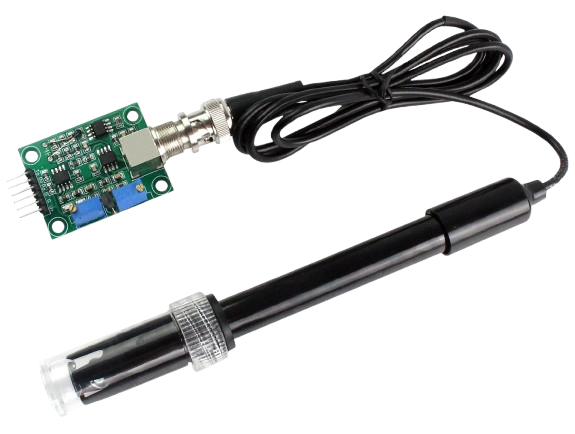
\includegraphics[width=\linewidth]{Imagem/sensorPh.png}
\end{minipage}
\begin{minipage}{0.32\linewidth}
    \centering
    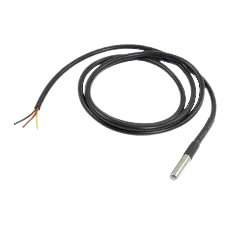
\includegraphics[width=\linewidth]{Imagem/sensorTemperatura.png}
\end{minipage}
\end{center}
\end{frame}

\section{Metodologia}
\begin{frame}{Metodologia}
\justifying
\begin{figure}[!htb]
\centering
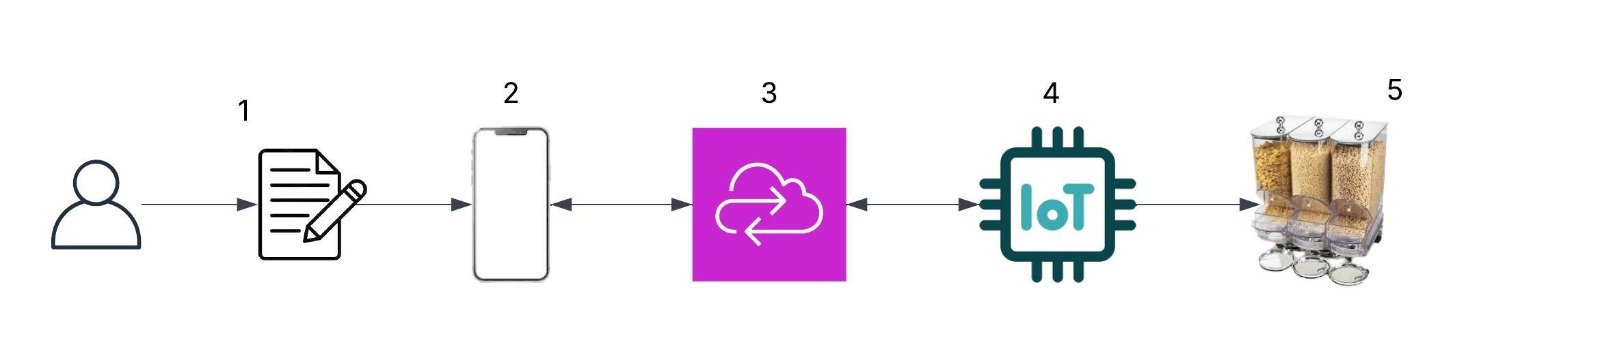
\includegraphics[width=\linewidth]{Imagem/Fluxograma.jpeg}
\end{figure}
\end{frame}

\section{Metodologia}
\begin{frame}{Metodologia}
\justifying
Tecnologias utilizadas para a aplicação
\vspace{0.5cm}

\begin{center}
\begin{minipage}{0.18\linewidth}
    \centering
    
\includegraphics[width=\linewidth]{Imagem/React-icon.svg.png}
\end{minipage}
\hspace{10pt}
\begin{minipage}{0.18\linewidth}
    \centering
    
\includegraphics[width=\linewidth]{Imagem/Node.js_logo.svg.png}
\end{minipage}
\hspace{10pt}
\begin{minipage}{0.18\linewidth}
    \centering
    
\includegraphics[width=\linewidth]{Imagem/pwa.png}
\end{minipage}
\hspace{10pt}
\begin{minipage}{0.18\linewidth}
    \centering
    
\includegraphics[width=\linewidth]{Imagem/mongoatlas.png}
\end{minipage}
\end{center}
\end{frame}


\section{Apresentação Prática}
\begin{frame}{Apresentação Prática}
\justifying
\begin{itemize}
    \item Sistema PWA desenvolvido
    \item Circuito IoT
\end{itemize}
\end{frame}

\section{Resultados Preliminares}
\begin{frame}{Resultados Preliminares}
\justifying
\begin{itemize}
    \item Desenvolvimento PWA em React
    \item Integração do circuito IoT
    \item Hospedagem da aplicação na nuvem
\end{itemize}
\end{frame}

\section{Conclusão}
\begin{frame}{Conclusão}
\justifying
\end{frame}

\end{document}
